% igs2eguide.tex
% v2.00 12-jun-08

\NeedsTeXFormat{LaTeX2e}

% The default is for Journal of Glaciology, one column, A4 paper. The other options are listed below:

% \documentclass{igs}
  \documentclass[twocolumn]{igs}
% \documentclass[annals]{igs}
% \documentclass[annals,twocolumn]{igs}

% \documentclass[letterpaper]{igs}
% \documentclass[twocolumn,letterpaper]{igs}
% \documentclass[annals,letterpaper]{igs}
% \documentclass[annals,twocolumn,letterpaper]{igs}

% when submitting your article for review, use one
% of the following two options:

% \documentclass[review]{igs}
% \documentclass[annals,review]{igs}

  \usepackage{igsnatbib}
  \usepackage{stfloats}

% check if we are compiling under latex or pdflatex
  \ifx\pdftexversion\undefined
    \usepackage[dvips]{graphicx}
  \else
    \usepackage[pdftex]{graphicx}
  \fi

% the default is for unnumbered section heads
% if you really must have numbered sections, remove
% the % from the beginning of the following command
% and insert the level of sections you wish to be
% numbered (up to 4):

% \setcounter{secnumdepth}{2}

\begin{document}

\title[IGS \LaTeXe\ guide]{Authors' guide to the
  IGS \LaTeXe\ class file}

\author[Woollatt and others]{Ali J. WOOLLATT,$^1$
  Craig BAXTER,$^2$\protect\thanks{Present address:
  Center for Glaciology, Institute of Geography and
  Earth Sciences, University of Wales, Aberystwyth
  SY23 3DB, UK.}\ \ Linda GORMAN,$^2$ Christine
  BUTLER,$^{3}$ Magn\'us M. MAGN\'USSON$^1$}

\affiliation{%
$^1$International Glaciological Society, Scott
  Polar Research Institute, Lensfield Road,
  Cambridge CB2 1ER, UK\\
E-mail: ali@igsoc.org\\
$^2$Climate Change Institute, University of Maine,
  303 Bryand Global Sciences Center, Orono,
  ME 04469-5790, USA\\
$^3$Institute of Geological and Nuclear Sciences
  Ltd, PO Box 30368, Lower Hutt, New Zealand}

\abstract{The design for the \emph{Journal/Annals of Glaciology} has been implemented as a \LaTeXe\ class file and is derived from article.cls. It is intended that authors use the class file in two-column format to check that mathematical equations fit the measure, but that submitted papers are in one-column format. The \emph{Journal/Annals of Glaciology} are printed in Optima. However, submissions using Computer Modern are fine. If you have any problems using the class file, please email Ali Woollatt at the above address, attaching your tex, log, cls, sty, bib, bbl, bst and any additional sty files you are using. The abstract should be less than 200 words and one paragraph long.}

\maketitle

\section{Using the IGS class file}
The IGS \LaTeXe\ guide has examples of most environments authors are likely to come across. The title page contains some new environments, e.g. affiliation and abstract, illustrated below. Papers should be divided into unnumbered sections with short section headings. SI units and internationally recognized systems of abbreviation should be used throughout. The \TeX\ file should be named to reflect your paper number, i.e. 06J015.tex.

\subsection{Additional packages supplied with igs.cls}
The distribution package contains 19 files, namely\\*[0.5\baselineskip]
\begin{tabular}{@{}ll}
igs.cls & IGS class file\\
igs.bst & IGS bibliography style file\\
igsnatbib.sty & IGS style file for citations\\
igsupmath.sty & IGS style file for upright Greek characters\\
igs2eguide.tex & IGS \LaTeX\ guide\\
igs2eguide.bib & sample \textsc{Bib}\TeX\ database\\
igs2eguide.pdf & pdf file of this guide\\
amsbsy.sty & style file called in by igsupmath.sty\\
amsgen.sty & \hskip 65pt\texttt{"}\\
amssymb.sty & accesses AMS fonts \verb"msam" and \verb"msbm"\\
amsfonts.sty & style file called in by amssymb.sty\\
fig01.eps & figure 1\\
fig02.eps & figure 2\\
graphicx.sty & graphics style file\\
lineno.sty & style file required for [review] option\\
edtable.sty & \hskip 65pt\texttt{"}\\
ednmath0.sty & \hskip 65pt\texttt{"}\\
ltabptch.sty & \hskip 65pt\texttt{"}\\
stfloats.sty & style file to enable double-column floats\\
             & to fall at the bottom of pages
\end{tabular}

\subsection{Typesetting the title page}

In the IGS design, shortened versions of the title and authors are used in the running head. The shortened version is typeset in square braces immediately after the \verb"\title" and \verb"\author" commands (see below). The order in which the following elements appear may be crucial, i.e. \verb"\maketitle" must be the last command before your paper commences. The default style is for Journal of Glaciology, one column, A4 paper. The other options are listed below. Authors using letterpaper size can use the letterpaper option, which reduces the number of lines on the page from 63 to 59 (the text width remains the same). Be aware that using letterpaper will fractionally lengthen your article. This guide was typeset using the following code:
\begin{verbatim}

% \documentclass{igs}
  \documentclass[twocolumn]{igs}
% \documentclass[annals]{igs}
% \documentclass[annals,twocolumn]{igs}

% \documentclass[letterpaper]{igs}
% \documentclass[twocolumn,letterpaper]{igs}
% \documentclass[annals,letterpaper]{igs}
% \documentclass[annals,twocolumn,letterpaper]{igs}

% when submitting your article for review, use one
% of the following two options:

% \documentclass[review]{igs}
% \documentclass[annals,review]{igs}

  \usepackage{igsnatbib}
  \usepackage{stfloats}

% check if we are compiling under latex or pdflatex
  \ifx\pdftexversion\undefined
    \usepackage[dvips]{graphicx}
  \else
    \usepackage[pdftex]{graphicx}
  \fi

% the default is for unnumbered section heads
% if you really must have numbered sections, remove
% the % from the beginning of the following command
% and insert the level of sections you wish to be
% numbered (up to 4):

% \setcounter{secnumdepth}{2}

\begin{document}

\title[IGS \LaTeXe\ guide]{Authors' guide to the
  IGS \LaTeXe\ class file}

\author[Woollatt and others]{Ali J. WOOLLATT,$^1$
  Craig BAXTER,$^2$\protect\thanks{Present address:
  Center for Glaciology, Institute of Geography and
  Earth Sciences, University of Wales, Aberystwyth
  SY23 3DB, UK.}\ \ Linda GORMAN,$^2$ Christine
  BUTLER,$^{3}$ Magn\'us M. MAGN\'USSON$^1$}

\affiliation{%
$^1$International Glaciological Society, Scott
  Polar Research Institute, Lensfield Road,
  Cambridge CB2 1ER, UK\\
E-mail: ali@igsoc.org\\
$^2$Climate Change Institute, University of Maine,
  303 Bryand Global Sciences Center, Orono,
  ME 04469-5790, USA\\
$^3$Institute of Geological and Nuclear Sciences
  Ltd, PO Box 30368, Lower Hutt, New Zealand}

\abstract{The design for the \emph{Journal/Annals
  of Glaciology} has been implemented as a \LaTeXe\
  class file...}

\maketitle

\section{Using the IGS class file}

\end{verbatim}

\subsection{Lists}
The IGS class file provides for numbered (\verb"enumerate") and unnumbered (\verb"itemize") lists. Nested lists are not encouraged. The default numbering system is 1., 2., 3., etc., please do not change this unless there is a good reason. The IGS design removes bullet points from unnumbered lists.

\subsection{User-defined macros}
If you define your own macros you must ensure that their names do not conflict with any existing macros in plain \TeX\ or \LaTeXe. They should be placed in the preamble to your input file, between \verb"\documentclass" and \verb"\begin{document}". You can check if the macro name is already in use by typing \verb"\show\<macro_name>".

\begin{table}% table1, one column
\caption{One-column table captions will extend beyond
  the rules in two-column format. Do not try to adjust!
  Table captions do not have full points at the end}
\label{period}
\begin{minipage}{86mm}% you only need this line if you
  % have a table footnote
\begin{tabular}{@{}lcc}\hline
Period\footnote{A table must be inside a \texttt{minipage}
  environment if it includes table footnotes.}
  & Surface elevation change
  & Emergence velocity\\ \hline
1975--85   & $-0.50$ & 0.43\\
1986--2002 & $-1.03$ & 0.32\\
Difference & $-0.53$ & \llap{$-$}0.11\\
\end{tabular}
\end{minipage}% you only need this line if you have a
  % table footnote
\vspace\baselineskip\hrule % to separate verbatim from table
\vspace\baselineskip
\begin{verbatim}
\begin{table}% table1, one column
\caption{One-column table captions will extend beyond
  the rules in two-column format. Do not try to adjust!
  Table captions do not have full points at the end}
\label{period}
\begin{minipage}{86mm}% you only need this line if you
  % have a table footnote
\begin{tabular}{@{}lcc}\hline
Period\footnote{A table must be inside a \texttt{minipage}
  environment if it includes table footnotes.}
  & Surface elevation change
  & Emergence velocity\\ \hline
1975--85   & $-0.50$ & 0.43\\
1986--2002 & $-1.03$ & 0.32\\
Difference & $-0.53$ & \llap{$-$}0.11\\
\end{tabular}
\end{minipage}% you only need this line if you have a
  % table footnote
\end{table}
\end{verbatim}
\vspace\baselineskip\hrule % to separate verbatim from text
\end{table}

\subsection{Tables}

Tables may be typeset in either one- or two-column format. To typeset two-column format, add asterisks\\
(\verb"\begin{table*}...\end{table*}") as shown in Table~\ref{seasonal}. We may change the format in-house if necessary. Please note that if you choose to refer to tables using labels, \verb"\caption" must precede \verb"\label", as in standard \LaTeX. Vertical rules are not house-style and will be removed. Note the use of the minipage environment in Table~\ref{period} which enables table footnotes to be output. If the table is two column, use \texttt{\{178mm\}} instead of \texttt{\{86mm\}} on line~6. The source code for Tables~\ref{period} and~\ref{seasonal} is shown immediately below the tables.

\begin{table*}[b]% table2, two column, place at bottom of page
\caption{Two-column table. Seasonal and annual SAT trends ($^\circ$C\,decade$^{-1}$) in the Arctic}
\label{seasonal}
% the following illustrates how to align columns on decimal points
% since all numbers are the same width in LaTeX, redefine a ? to take up the width of a number
% do not use if your table contains a genuine ?
\catcode`\?=\active \gdef?{\setbox0=\hbox{0}\hbox to\wd0{}}%
\setlength\tabcolsep{2.5pt}% column separation reduced from the default 6pt so the table fits the measure
\begin{tabular}{@{}l@{\hspace{20pt}}ccccc@{\hspace{20pt}}ccccc}\hline
Area                 & \multicolumn{5}{c}{1951--2005} & \multicolumn{5}{c}{1976--2005}\\[5pt]
                     & Dec.--Feb.     & Mar.--May   & Jun.--Aug.  & Sep.--Nov.     & Annual
                     & Dec.--Feb.     & Mar.--May   & Jun.--Aug.  & Sep.--Nov.     & Annual\\ \hline
Atlantic region      & 0.09           & 0.29 & 0.10 & 0.09 & 0.15 & 0.470 & ??0.60 & 0.45 & 0.53 & 0.59\\
Siberian region      & 0.12           & 0.29 & 0.04 & 0.17 & 0.16 & 0.08? & ??0.69 & 0.29 & 0.59 & 0.48\\
Pacific region       & 0.45           & 0.46 & 0.25 & 0.26 & 0.35 & 0.712 & ??1.08 & 0.27 & 0.66 & 0.52\\
Canadian region      & 0.16           & 0.12 & 0.14 & 0.30 & 0.18 & 0.20? & ??0.52 & 0.48 & 0.94 & 0.53\\
Baffin Bay region    & \llap{$-$}0.02 & 0.10 & 0.00 & 0.15 & 0.02 & 0.33? & ??0.62 & 0.51 & 0.80 & 0.57\\
Arctic 1             & 0.16           & 0.21 & 0.12 & 0.20 & 0.18 & 0.36? & 200.65 & 0.42 & 0.74 & 0.54\\
Arctic 2             & 0.22           & 0.29 & 0.14 & 0.14 & 0.19 & 0.38? & ??0.60 & 0.40 & 0.51 & 0.45\\
Arctic 3             & 0.28           & 0.31 & 0.14 & 0.13 & 0.21 & 0.42? & ?40.53 & 0.41 & 0.42 & 0.43\\
NH ($\mathrm{land}
  + \mathrm{ocean}$) & 0.13           & 0.13 & 0.10 & 0.10 & 0.12 & 0.27? & ??0.24 & 0.25 & 0.25 & 0.25\\
\hline
\end{tabular}
% turn off the category change, otherwise the ? won't appear in the verbatim environment below
\catcode`\?=11%
\vspace{0.25\baselineskip}
\begin{verbatim}
\begin{table*}[b]% table2, two column, place at bottom of page
\caption{Two-column table. Seasonal and annual SAT trends ($^\circ$C\,decade$^{-1}$) in the Arctic}
\label{seasonal}
% the following illustrates how to align columns on decimal points
% since all numbers are the same width in LaTeX, redefine a ? to take up the width of a number
% do not use if your table contains a genuine ?
\catcode`\?=\active \gdef?{\setbox0=\hbox{0}\hbox to\wd0{}}%
\setlength\tabcolsep{2.5pt}% column separation reduced from the default 6pt so the table fits the measure
\begin{tabular}{@{}l@{\hspace{20pt}}ccccc@{\hspace{20pt}}ccccc}\hline
Area                 & \multicolumn{5}{c}{1951--2005} & \multicolumn{5}{c}{1976--2005}\\[5pt]
                     & Dec.--Feb.     & Mar.--May   & Jun.--Aug.  & Sep.--Nov.     & Annual
                     & Dec.--Feb.     & Mar.--May   & Jun.--Aug.  & Sep.--Nov.     & Annual\\ \hline
Atlantic region      & 0.09           & 0.29 & 0.10 & 0.09 & 0.15 & 0.470 & ??0.60 & 0.45 & 0.53 & 0.59\\
Siberian region      & 0.12           & 0.29 & 0.04 & 0.17 & 0.16 & 0.08? & ??0.69 & 0.29 & 0.59 & 0.48\\
Pacific region       & 0.45           & 0.46 & 0.25 & 0.26 & 0.35 & 0.712 & ??1.08 & 0.27 & 0.66 & 0.52\\
Canadian region      & 0.16           & 0.12 & 0.14 & 0.30 & 0.18 & 0.20? & ??0.52 & 0.48 & 0.94 & 0.53\\
Baffin Bay region    & \llap{$-$}0.02 & 0.10 & 0.00 & 0.15 & 0.02 & 0.33? & ??0.62 & 0.51 & 0.80 & 0.57\\
Arctic 1             & 0.16           & 0.21 & 0.12 & 0.20 & 0.18 & 0.36? & 200.65 & 0.42 & 0.74 & 0.54\\
Arctic 2             & 0.22           & 0.29 & 0.14 & 0.14 & 0.19 & 0.38? & ??0.60 & 0.40 & 0.51 & 0.45\\
Arctic 3             & 0.28           & 0.31 & 0.14 & 0.13 & 0.21 & 0.42? & ?40.53 & 0.41 & 0.42 & 0.43\\
NH ($\mathrm{land}
  + \mathrm{ocean}$) & 0.13           & 0.13 & 0.10 & 0.10 & 0.12 & 0.27? & ??0.24 & 0.25 & 0.25 & 0.25\\
\hline
\end{tabular}
\end{table*}
\end{verbatim}
\vspace\baselineskip\hrule % to separate verbatim from text
\end{table*}


\subsection{Figures}

Figures may be typeset in either one- or two-column format. One-column format allows up to 86$\,$mm (e.g. Fig.~\ref{tracks}); two-column format up to 178$\,$mm (e.g. Fig.~\ref{filters}). To typeset two-column format, add asterisks (\verb"\begin{figure*}...\end{figure*}") as shown in Figure~\ref{filters}. We may change the format in-house if necessary. Please note that if you choose to refer to figures using labels, \verb"\caption" must precede \verb"\label", as in standard \LaTeX.

In addition, figures should be eps, ai (illustrator), ps, tif, psd, \emph{not} jpeg. Use strong black lines (avoid tinting if possible) and SI units in labels. Lettering should ideally be Optima to match the final typeface; Ariel or a similar sans serif font for a second choice. Aim to have the final-size lettering at 9pt, if possible. Figures should not be in boxes. The source code for Figures~\ref{tracks} and~\ref{filters} is shown immediately below the figures.


\subsection{Equations}

We are including some complex equations as examples. Equations should be checked for width using the \verb"[twocolumn]" option. Note the use of arrays in the following equation:
\begin{equation}
\label{arrayexample}
\alpha_{t_2}= \left\{%
  \begin{array}{ll}
    \alpha_{t_1} - a_1 [\ln (T+1)]
      \mathrm{e}^{(a_2\sqrt{n})}
      & \mbox{$n_\mathrm{d} > 0\enskip$ and
      $\enskip T > 0$}\\
    \alpha_{t_1} - a_3 \mathrm{e}^{(a_2\sqrt{n})}
      & \mbox{$n_\mathrm{d} > 0\enskip$ and
      $\enskip T < 0$}\\
    \alpha_{t_1} + a_4 P_\mathrm{s}
      & \mbox{$n_\mathrm{d} = 0$}
  \end{array}
\right.
\end{equation}
Equation~(\ref{arrayexample}) above used the following code:
\begin{verbatim}

\begin{equation}
\label{arrayexample}
\alpha_{t_2}= \left\{%
  \begin{array}{ll}
    \alpha_{t_1} - a_1 [\ln (T+1)]
      \mathrm{e}^{(a_2\sqrt{n})}
      & \mbox{$n_\mathrm{d} > 0\enskip$ and
      $\enskip T > 0$}\\
    \alpha_{t_1} - a_3 \mathrm{e}^{(a_2\sqrt{n})}
      & \mbox{$n_\mathrm{d} > 0\enskip$ and
      $\enskip T < 0$}\\
    \alpha_{t_1} + a_4 P_\mathrm{s}
      & \mbox{$n_\mathrm{d} = 0$}
  \end{array}
\right.
\end{equation}

\end{verbatim}
Equations should be aligned on the equals signs where possible. Equations that extend beyond the one-column measure should be turned over before an operator. Note the \verb"\skew4" command below which moves the bar over the $R$ to the right. The value generally varies between \verb"\skew1" and \verb"\skew5".
\begin{eqnarray}
\label{eqnarrayexample}
l_c &=& l_0 \left(\frac{\skew4\bar R_m}{R} \right)^2
  \psi^{\frac{P}{P_0\cos Z}}\nonumber\\
    &&  \mbox{}\times [\cos\beta\, \cos Z
    + \sin\beta\,\sin Z\,\cos(\psi_\mathrm{sun}
    - \psi_\mathrm{slope})]
\end{eqnarray}
Equation~(\ref{eqnarrayexample}) above used the following code:
\begin{verbatim}

\begin{eqnarray}
\label{eqnarrayexample}
l_c &=& l_0 \left(\frac{\skew4\bar R_m}{R} \right)^2
  \psi^{\frac{P}{P_0\cos Z}}\nonumber\\
    &&  \mbox{}\times [\cos\beta\, \cos Z
    + \sin\beta\,\sin Z\,\cos(\psi_\mathrm{sun}
    - \psi_\mathrm{slope})]
\end{eqnarray}

\end{verbatim}

\subsection{Typesetting upright Greek characters}

The \verb"igsupmath" package provides macros for upright lower-case Greek (\verb"\ualpha"--\verb"\uxi"), and for bold lower-case Greek (\verb"\ubalpha"--\verb"\ubxi"). The bold upright symbol \verb"\eta" has to be treated differently, in this case use \verb"\uboldeta".

To use the \verb"igsupmath" package, you need to have the AMS \verb"eurm/b" fonts installed.

The AMS packages are supplied from the AMS\,\LaTeX\ distribution. If you already have the AMS\,\LaTeX\ distribution installed, you can safely delete the \verb"ams*.sty" files (it is worth checking if the supplied files are newer). If you do not have them already, the latest AMS Fonts/AMS\,\LaTeX\ distributions can be found at http://www.ctan.org/.

For upright characters add a \verb"u", and for upright bold characters, \verb"ub", e.g.\\*[0.5\baselineskip]
\begin{tabular}{@{}ll@{\hspace{40pt}}ll}
$\ualpha$   & \verb"$\ualpha$"      &    $\ubalpha$ & \verb"$\ubalpha$"\\
$\ubeta$    & \verb"$\ubeta$"       &    $\ubbeta$ & \verb"$\ubbeta$"\\
$\ugamma$   & \verb"$\ugamma$"      &    $\ubgamma$ & \verb"$\ubgamma$"\\
$\udelta$   & \verb"$\udelta$"      &    $\ubdelta$ & \verb"$\ubdelta$"
\end{tabular}\\[0.5\baselineskip]
Authors who do not have this font are requested to key their articles using the commands above. The characters will be substituted automatically by the typesetter.

\subsection{Typesetting the partial symbol}

The \verb"igsupmath" package also provides \verb"\upartial" and \verb"\ubpartial".

Provided you have the AMS fonts, you can use the style file igsupmath.sty to typeset the partial symbol, e.g.\\*[0.5\baselineskip]
\begin{tabular}{@{}ll@{\hspace{40pt}}ll}
$\upartial$ & \verb"$\upartial$"    &    $\ubpartial$ & \verb"$\ubpartial$"\\
\end{tabular}


\subsection{Marginal notes}

The IGS class file\marginpar{Editor! Help!} redefines the \LaTeX\ command \verb"\marginpar". If you wish to add a marginal note such as the one alongside this text, you would key \verb"\marginpar{Editor! Help!}". Marginal notes will be removed before printing.

\subsection{References}

All citations in text should include the author name(s) and the year of publication (e.g. `Smith, 1999'; `Smith and Jones, 2000'; `Smith and others, 2003') and have an entry in the reference list.

References should:
\begin{itemize}
\item be short;
\item be complete and accurate;
\item be arranged in alphabetical order by first author's surname;
\item include too much rather than too little information;
\item include works accepted but not published as `in press';
\item not include personal communications, unpublished data or manuscript in preparation or submitted for publication, data published on the web (these should be included in the text).
\end{itemize}

\begin{figure}%fig01, one column
\centering{\includegraphics[width=80mm]{fig01.eps}}
\caption{One-column figures should be $\leq$86$\,$mm.
Good artwork can make or break a paper.}
\label{tracks}
\vspace\baselineskip\hrule % to separate figure from verbatim
\vspace\baselineskip
\begin{verbatim}
\begin{figure}%fig01, one column
\centering{\includegraphics[width=80mm]{fig01.eps}}
\caption{One-column figures should be $\leq$86$\,$mm.
Good artwork can make or break a paper.}
\label{tracks}
\end{figure}
\end{verbatim}
\vspace\baselineskip\hrule % to separate verbatim from text
\end{figure}

\subsubsection{Automatic references using \textsc{Bib}\upshape{\TeX}}

To generate automatic references from a bib database, you must first place the following two commands where you would like the references to appear (normally at the end of your paper, before \verb"\end{document}"
%
\begin{verbatim}

\bibliography{igs2eguide}% reads igs2eguide.bib
\bibliographystyle{igs}
  % imposes IGS bibliography style on output

\end{verbatim}
%
Next, run your paper through \LaTeX\ twice, run \textsc{Bib}\TeX, then run it through \LaTeX\ once again. This series of runs will generate a file called igs2eguide.bbl (in the case of this guide), which will then be included by the first of the two commands above.

If you have cited 9 references from the bib database, e.g. \citep{Huybrechts92}, \citep{Blatter95,Pfender99}, \citep{Henner00}, \citep{USN:1966}, \citep{Krimmel:2000a}, \citep{johnsen77}, \citep{Braun01} and \citep{dahl-jensen93}, the output will be just those 9 references and they will appear at the end of the article.

\paragraph{Citations using natbib commands}
Note that the standard natbib style file has been modified to fall into line with IGS style. The modified style file is called igsnatbib.sty (included in this distribution), and works exactly the same as natbib.sty. The default IGS house style is \citep{Blatter95}. The following combinations are also available -- refer to the natbib documentation if you require any further explanation:\\*[0.5\baselineskip]
\begin{tabular}{@{}l@{\hskip -44pt}l}
\citep{Blatter95}
    & \verb"\citep{Blatter95}"\\
\citep[see][p.$\,$34]{Blatter95}\\
    & \verb"\citep[see][p.$\,$34]{Blatter95}"\\
\citep[e.g.][]{Blatter95}
    & \verb"\citep[e.g.][]{Blatter95}"\\
\citep[section~2.3]{Blatter95}\\
    & \verb"\citep[section~2.3]{Blatter95}"\\
\citep{Huybrechts92, Blatter95}\\
    &  \verb"\citep{Huybrechts92, Blatter95}"\\
\cite{Huybrechts92, Blatter95}\\
    &  \verb"\cite{Huybrechts92, Blatter95}"\\
\citealt{Braun01}
    & \verb"\citealt{Braun01}"\\
\cite{Blatter95}
    & \verb"\cite{Blatter95}"\\
\citealp{Huybrechts92}
    & \verb"\citealp{Huybrechts92}"\\
\citeauthor{Huybrechts92}
    & \verb"\citeauthor{Huybrechts92}"\\
\citeyearpar{Huybrechts92}
    & \verb"\citeyearpar{Huybrechts92}"\\
\citeyear{Huybrechts92}
    & \verb"\citeyear{Huybrechts92}"
\end{tabular}

\begin{figure*}%fig02, two column
\centering{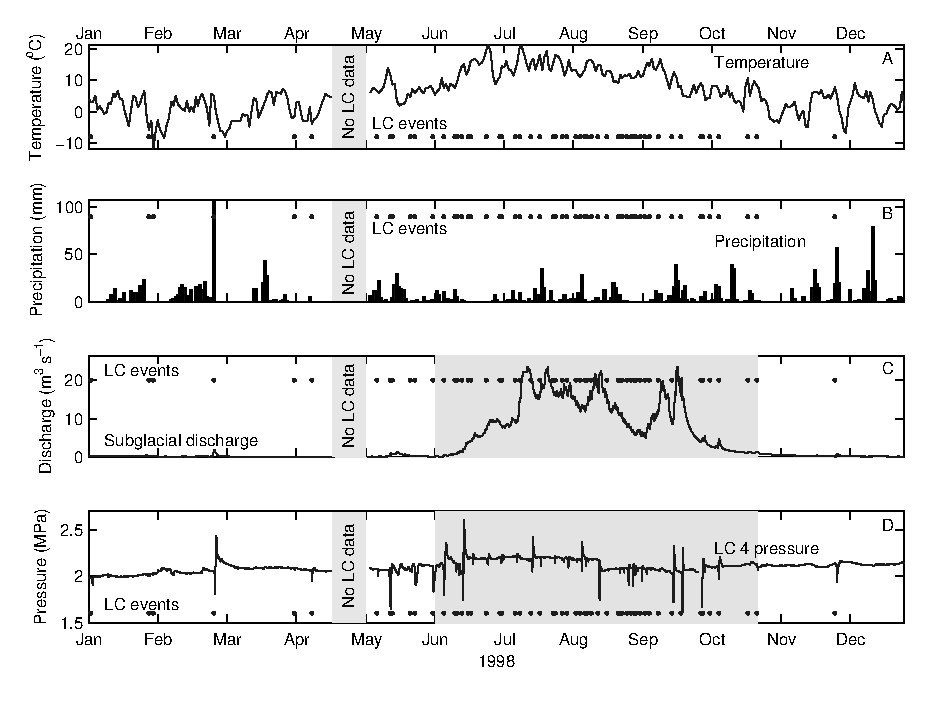
\includegraphics[width=140mm]{fig02.eps}}
\caption{Two-column figures should be $\leq$178$\,$mm. SSA reconstructed components found by projecting the
  SSA filters found using the whole 2000 traces in Figure~4, on trace number 1, ordered by magnitude of
  variance accounted for in the radar trace.}
\label{filters}
\vspace\baselineskip\hrule % to separate figure from verbatim
\vspace\baselineskip
\begin{verbatim}
\begin{figure*}%fig02, two column
\centering{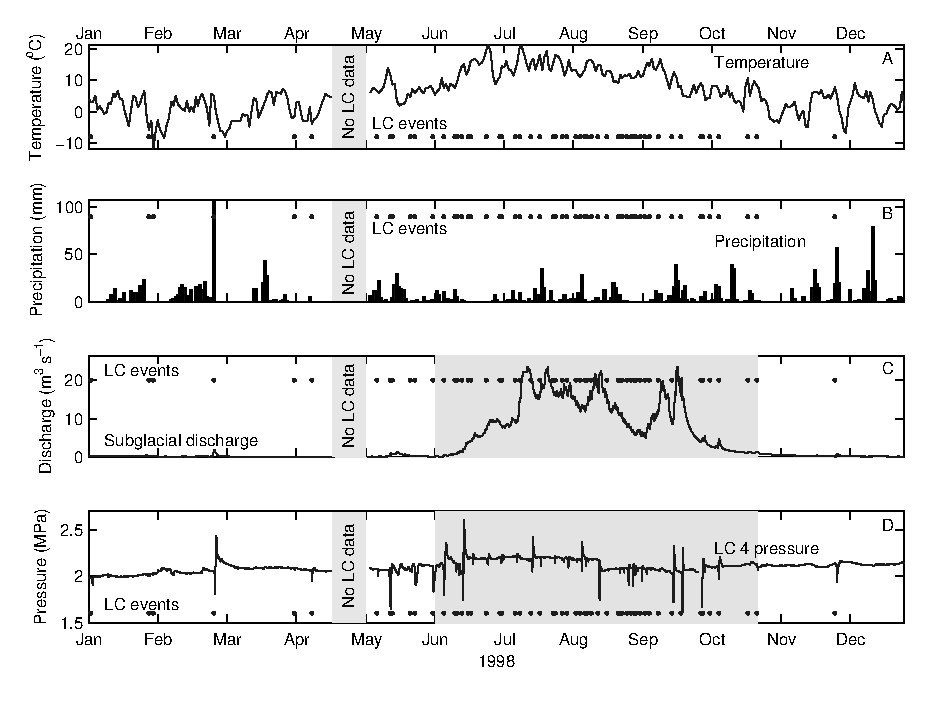
\includegraphics[width=140mm]{fig02.eps}}
\caption{Two-column figures should be $\leq$178$\,$mm. SSA reconstructed components found by projecting the
  SSA filters found using the whole 2000 traces in Figure~4, on trace number 1, ordered by magnitude of
  variance accounted for in the radar trace.}
\label{filters}
\end{figure*}
\end{verbatim}
\vspace\baselineskip\hrule % to separate verbatim from text
\end{figure*}

\subsubsection{Manual references}
Authors not using the bibligraphy style file igs.bst can produce the same output at the end of the guide by typing the references along the following lines:

\begin{verbatim}

\begin{thebibliography}{9}
\expandafter\ifx\csname natexlab\endcsname\relax
  \def\natexlab#1{#1}\fi
\expandafter\ifx\csname selectlanguage\endcsname\relax
  \def\selectlanguage#1{\relax}\fi

\bibitem[Blatter, 1995]{Blatter95}
Blatter, H., 1995. Velocity and stress fields in
  grounded glaciers: a simple algorithm for
  including deviatoric stress gradients,
  {\em J.~Glaciol.\/}, {\bf 41}(138), 333--344.

\bibitem[Braun and others, 2001]{Braun01}
Braun, M., {J.C.} {Sim\~{o}es}, S.~Vogt,
  {U.F.} Bremer, H.~Saurer and {F.E.} Aquino,
  2001. A new satellite image map of King George
  Island (South Shetland Islands, Antarctica),
  {\em Polarforschung\/}, {\bf 71}(1/2), 47--48.

\bibitem[Dahl-Jensen and others, 1993]{dahl-jensen93}
Dahl-Jensen, D., S.J. Johnsen, C.U. Hammer,
  H.B. Clausen and J.~Jouzel, 1993. Past
  accumulation rates derived from observed annual
  layers in the {GRIP} ice core from {S}ummit,
  central {G}reenland., Peltier, W.R., ed., Ice
  in the Climate System, Springer-Verlag, Berlin
  Heidelberg, Germany, 517--532.

\bibitem[Huybrechts, 1992]{Huybrechts92}
Huybrechts, P., 1992. The Antarctic ice sheet and
  environmental change: a three-dimensional
  modelling study, vol.~99 of {\em Berichte zur
  Polarforschung\/}, Alfred-Wegener-Institut
  Bremerhaven.

\bibitem[Johnsen, 1977]{johnsen77}
Johnsen, S.J., 1977. Stable isotope homogenization
  of polar firn and ice, Proceedings of the
  Grenoble Symposium on {I}sotopes and
  {I}mpurities in {S}now and {I}ce, Grenoble,
  Aug./Sep. 1975, IAHS Publ., no. 118, 210--219.

\bibitem[Krimmel, 2000]{Krimmel:2000a}
Krimmel, R.M., 2000. {Water, ice, and
  meteorological measurements at South Cascade
  Glacier, Washington, 1986--1991 balance years},
  {\em {USGS Water-Resourc. Invest. Rep.
  00-4006}\/}, 77 p.

\bibitem[Pfender, 1999]{Pfender99}
Pfender, M., 1999. Topographie und Glazialhydrologie
  von King George Island, Antarktis, (Master's
  thesis, Westf\"{a}lische Wilhelms-Universit\"{a}t
  M\"{u}nster).

\bibitem[Sand\-h\"ager, 2000]{Henner00}
Sand\-h\"ager, H., 2000. Quantifizierung
  eisdynamischer und massenhaushaltsrelevanter
  Basisgr\"{o}\ss en eines antarktischen
  Inlandeis-Schelfeis-Systems unter Einsatz eines
  numerischen Flie\ss modells, (PhD thesis,
  Westf\"{a}lische Wilhelms-Universit\"{a}t
  M\"{u}nster).

\bibitem[{United States Navy}, 1966]{USN:1966}
{United States Navy}, 1966. {Selected level
  temperatures and dew points for the Northern
  Hemisphere}, {Washington, DC, US Navy: Chief of
  Naval Operations}, {(Document NAVAIR 50-1C-52)}.

\end{thebibliography}

\end{verbatim}

\section{Acknowledgements}
The authors would like to thank J.~Amundson, E.~Bueler, A.~Clifton, G.~Flowers and R.~Greve for their constructive reviews of the IGS class file and guide. Thanks are also due to P.\,W. Daly who generated a new version of igs.bst.

% authors generating their own bbl file would uncomment the following two lines, and comment out/delete the references below:
% \bibliography{igs2eguide}% reads igs2eguide.bib
% \bibliographystyle{igs}  % imposes IGS bibliography style on output

% however, we are going to include igs2eguide.bbl here:

\begin{thebibliography}{9}
\expandafter\ifx\csname natexlab\endcsname\relax
  \def\natexlab#1{#1}\fi
\expandafter\ifx\csname selectlanguage\endcsname\relax
  \def\selectlanguage#1{\relax}\fi

\bibitem[Blatter, 1995]{Blatter95}
Blatter, H., 1995. Velocity and stress fields in
  grounded glaciers: a simple algorithm for
  including deviatoric stress gradients,
  {\em J.~Glaciol.\/}, {\bf 41}(138), 333--344.

\bibitem[Braun and others, 2001]{Braun01}
Braun, M., {J.C.} {Sim\~{o}es}, S.~Vogt,
  {U.F.} Bremer, H.~Saurer and {F.E.} Aquino,
  2001. A new satellite image map of King George
  Island (South Shetland Islands, Antarctica),
  {\em Polarforschung\/}, {\bf 71}(1/2), 47--48.

\bibitem[Dahl-Jensen and others, 1993]{dahl-jensen93}
Dahl-Jensen, D., S.J. Johnsen, C.U. Hammer,
  H.B. Clausen and J.~Jouzel, 1993. Past
  accumulation rates derived from observed annual
  layers in the {GRIP} ice core from {S}ummit,
  central {G}reenland., Peltier, W.R., ed., Ice
  in the Climate System, Springer-Verlag, Berlin
  Heidelberg, Germany, 517--532.

\bibitem[Huybrechts, 1992]{Huybrechts92}
Huybrechts, P., 1992. The Antarctic ice sheet and
  environmental change: a three-dimensional
  modelling study, vol.~99 of {\em Berichte zur
  Polarforschung\/}, Alfred-Wegener-Institut
  Bremerhaven.

\bibitem[Johnsen, 1977]{johnsen77}
Johnsen, S.J., 1977. Stable isotope homogenization
  of polar firn and ice, Proceedings of the
  Grenoble Symposium on {I}sotopes and
  {I}mpurities in {S}now and {I}ce, Grenoble,
  Aug./Sep. 1975, IAHS Publ., no. 118, 210--219.

\bibitem[Krimmel, 2000]{Krimmel:2000a}
Krimmel, R.M., 2000. {Water, ice, and
  meteorological measurements at South Cascade
  Glacier, Washington, 1986--1991 balance years},
  {\em {USGS Water-Resourc. Invest. Rep.
  00-4006}\/}, 77 p.

\bibitem[Pfender, 1999]{Pfender99}
Pfender, M., 1999. Topographie und Glazialhydrologie
  von King George Island, Antarktis, (Master's
  thesis, Westf\"{a}lische Wilhelms-Universit\"{a}t
  M\"{u}nster).

\bibitem[Sand\-h\"ager, 2000]{Henner00}
Sand\-h\"ager, H., 2000. Quantifizierung
  eisdynamischer und massenhaushaltsrelevanter
  Basisgr\"{o}\ss en eines antarktischen
  Inlandeis-Schelfeis-Systems unter Einsatz eines
  numerischen Flie\ss modells, (PhD thesis,
  Westf\"{a}lische Wilhelms-Universit\"{a}t
  M\"{u}nster).

\bibitem[{United States Navy}, 1966]{USN:1966}
{United States Navy}, 1966. {Selected level
  temperatures and dew points for the Northern
  Hemisphere}, {Washington, DC, US Navy: Chief of
  Naval Operations}, {(Document NAVAIR 50-1C-52)}.

\end{thebibliography}

\appendix
\section{Appendix}

Start an appendix by typing \verb"\appendix\section{Appendix}". Appendices appear after the references. Equation numbers automatically start again with (\ref{appeqn}).
\begin{equation}
\label{appeqn}
 2\eta\kappa \frac{\partial \skew1\bar u}{\partial t} + \rho_{\mathrm r} g \skew1\bar u + D\kappa^4 \skew1\bar u = \skew3\bar\sigma_{zz}.
\end{equation}

\end{document}
